\chapter{Prueba de Concepto}
\label{ch:aplicacion}

\begin{quote}
	{\bf\textsc{Resumen:}} Este capítulo presenta la prueba de concepto realizada para la integración de Información Geográfica procedente de Ogíjares (Granada) mediante herramientas de la Web Semántica, en donde se estudian y proponen herramientas de la Web Semántica que se pueden utilizar para representar e integrar datos geoespaciales. 
\end{quote}



\section{Prueba de Concepto}

Como hemos comentado, uno de nuestros objetivos es estudiar las herramientas de la Web Semántica que se pueden utilizar para representar e integrar Información Geográfica, valorarlas y desarrollar una prueba de concepto. Contaremos con la presencia de herramientas destinadas a la generación (\texttt{QGIS} para permitir obtener la información de los \textit{Shapefile} a hojas de cálculo y \texttt{Protegé} para permitir llevar la información de los \textit{Shapefile} hacia documentos en formato \textit{RDF} de manera gráfica y más sencilla), consumo (\texttt{GraphBD} para permitir la visualización de archivos en formato \textit{RDF} y para realizar las consultas del lenguaje estándar de consulta geoespacial \textit{GEOSPARQL}) y visualización (\texttt{R} para permitir ubicar la información geográfica en un mapa interactivo mediante la libería \textit{Shiny}). Antes de iniciar el proceso, vamos a ver cómo obtener los datos geográficos con los que hacer la prueba de concepto.

\subsection{Obtención de la Información Geográfica}

Como hemos comentando a lo largo del presente trabajo, nuestro objetivo es integrar información geospacial. En la actualidad, disponemos de diversas fuentes oficiales y no oficiales que nos proporcionan mapas de calidad. No obstante, al hacer uso de Información Geográfica de España, es importante destacar dos fuentes principales:

\begin{itemize}
	\item \textbf{Instituto Geográfico Nacional (IGN)}, es la fuenta oficial para todo el territorio español y la descarga de mapas se puede realizar a través de la dirección \url{http://centrodedescargas.cnig.es/CentroDescargas/buscador.do#}.
	
	\item \textbf{Instituto de Estadística y Cartografía de Andalucía}, es la fuente oficial para todo el territorio andaluz y la descarga de mapas se puede realizar a través de la dirección \url{https://www.juntadeandalucia.es/institutodeestadisticaycartografia/bcadescargas/}.
\end{itemize}
 
Sin embargo, como vamos a trabajar con datos procedentes de la provincia de Granada, en concreto de mi pueblo Ogíjares, he optado por escoger los que nos proporciona el \textit{Instituto de Estadística y Cartografía de Andalucía} \cite{base-andalucia}. A continuación, se muestran los pasos para su obtención:

\begin{enumerate}
	\item La descarga se realiza a través de la plataforma del Instituto de Estadística y Cartografía de Andalucía, de la Consejería de Economía y Conocimiento (URL mencionada en el punto anterior). Una vez dentro, seleccionamos la opción \texttt{Base Cartográfica de Andalucía (2)} y escogemos \textit{Base Cartográfica de Andalucía (shape)} y buscamos el municipio de \textit{Ogíjares} (figura \ref{fig:obtencion-informacion}). Nos aparecerán varios cuadrantes, escogemos con el que nosotros queramos trabajar; yo me he descargado el cuadrante que aparece seleccionado.

	\begin{figure}[H]
		\centering
		\includegraphics[width=1\linewidth]{imagenes/capitulo4/obtencion-informacion}
		\caption{Portal del Instituto de Estadística y Cartografía de Andalucía}
		\label{fig:obtencion-informacion}
	\end{figure}

	\item La carpeta descargada contiene mapas de áreas muy diversas, las cuales hacen uso de la geometría punto, línea o área. 

	\item El fichero descargado para cada uno de los mapas tiene como formato \textit{Shapefile (sh)}, es el formato más usado para almacenar información geoespacial. El contenido o visualización del fichero se muestra en la figura \ref{fig:shp}. Se trata de un formato de archivos que almacena información no topológica con características espaciales de elementos geográficos \cite{tesis}. Estos archivos suelen requerir poco espacio de almacenamiento en disco y se pueden leer y escribir con facilidad. Además, soportan geometrías como puntos, líneas y polígonos, y los atributos son almacenados en un archivo de formato dBase. Un archivo shapefile, originario de Enviromental Systems Research Institute (ESRI), consiste de un archivo principal, un archivo de índice y una tabla dBase. 
	
	\begin{itemize}
		\item El archivo principal (*.shp) es un archivo de longitud variable en el que cada registro describe una forma con sus respectivos vértices. 
		\item El archivo de índice (*.shx) acompaña al archivo principal (*.shp) que almacena la posición de los Id. de entidades individuales en el archivo .shp 
		\item La tabla dBase (*.dbf) almacena la información  de atributos de las entidades. 
	\end{itemize}	

	Los diferentes archivos que componen el formato shapefile deben tener el mismo nombre cada uno con su respectiva extensión,como se aprecia en la figura \ref{fig:shapefile}:
	
	\begin{figure}[H]
		\centering
		\includegraphics[width=1\linewidth]{imagenes/capitulo2/shapefile}
		\caption{Archivos shape}
		\label{fig:shapefile}
	\end{figure}
	
	Los archivos Shapefile pueden ser visualizados a través de cualquier software GIS, en la figura \ref{fig:visualizar-shapefile} se visualiza un archivo Shapefile válido utilizando el software de análisis geoespacial QGIS. 
	
	\begin{figure}[H]
		\centering
		\includegraphics[width=1\linewidth]{imagenes/capitulo2/visualizar-shapefile}
		\caption{ Visualización Geográfica de las Edificaciones de Ogíjares en QGIS}
		\label{fig:visualizar-shapefile}
	\end{figure}

\end{enumerate}











 en concreto vamos a descargarnos la información referenciada a Ogíjares de la \textit{Base Cartográfica de Andalucía (2)} y seleccionar \textit{Base Cartográfica de Andalucía (shape)} (figura \ref{fig:obtencion-informacion}).





\newpage




Por otra parte, existen multitud de fuentes oficiales y no oficiales para la descarga de MDT de manera gratuita. (\textit{En el \texttt{Apéndice} se puede encontrar más información de otras fuentes para la descarga de éstos}). Sin embargo, como vamos a trabajar con datos procedentes de la provincia de Granada, he optado por escoger los que nos proporciona el \textit{Instituto de Estadística y Cartografía de Andalucía} \cite{Instituto-Andalucia}, en concreto vamos a analizar el MDT para la zona de Chauchina, como hemos comentado anteriormente. A continuación, se muestran los pasos para su obtención:


\begin{enumerate}

	
	\item El fichero descargado tiene como formato \textit{Tagged Image File Format (tif)}, formato básico para el modelado de datos ráster. El contenido o visualización del fichero se muestra en la figura \ref{fig:tif}.
	
	\begin{figure}[H]
		\centering
		\includegraphics[height=6.35cm]{imagenes/capitulo2/4_Paso3-Obtencion.png}
		\caption{Archivo \textit{tif} de la zona descargada}
		\label{fig:tif}
	\end{figure}	
\end{enumerate}

Gracias a este tipo de archivo podemos generar MDT secundarios: mapas de orientación, de pendiente, cuencas visuales o sencillos archivos de sombreado (\textit{hillshade}), materia prima con la que analizar el territorio. Es por ello que, una vez descargados nuestros datos, ya podemos llevar a cabo el análisis del mapa de sombras para el MDT. Primero lo realizaremos en R, seguidamente en QGIS y, por último, veremos la interacción entre ambas, dejando documentado el proceso, para así poder hacer la evaluación y comparación entre ambas herramientas.





\newpage

% Uso de la similitud semántica para la recuperación de información geoespacial: https://dialnet.unirioja.es/servlet/tesis?codigo=61960
% http://rua.ua.es/dspace/handle/10045/45811
% https://rua.ua.es/dspace/bitstream/10045/45811/1/tesis_machado_garcia.pdf

% http://www.ciw.cl/material/tw07arodriguez.pdf

% Semántica Geoespacial en la web: https://slideplayer.es/slide/10277009/

% https://nextweb.gnoss.com/busqueda/tag/geoespacial

% Para que es para acceder a datos espaciales en la web
% http://linkedgeodata.org/OnlineAccess
% http://linkedgeodata.org/sparql

% https://www.w3.org/community/geosemweb/wiki/Main_Page
% https://en.wikipedia.org/wiki/Semantic_Geospatial_Web
% https://www.opengeospatial.org/projects/initiatives/gswie
% http://www.personal.psu.edu/faculty/f/u/fuf1/Fonseca-Sheth.pdf

% https://www.researchgate.net/publication/283801501_Geospatial_Semantic_Web
% https://www.researchgate.net/publication/300494545_Geospatial_Data_Interoperability_Geography_Markup_Language_GML_Scalable_Vector_Graphics_SVG_and_Geospatial_Web_Services
% https://www.semanticscholar.org/paper/Supporting-Frameworks-for-the-Geospatial-Semantic-Abdelmoty-Smart/e3998c31905b0d9eebaceddad5040e940caa594a
% https://www.sciencedirect.com/science/article/pii/S1570826809000468

% https://www.mdpi.com/journal/ijgi/special_issues/geospatial_semantics

% Documentos Scholar sobre "geospatial semantic web": https://scholar.google.es/scholar?q=geospatial+semantic+web&hl=es&as_sdt=0&as_vis=1&oi=scholart

% http://www.irisa.fr/LIS/ferre/sparklis/?title=Core%20English%20DBpedia&endpoint=http%3A//servolis.irisa.fr/dbpedia/sparql&sparklis-query=%5BVId%5DReturn%28Det%28An%281%2CModif%28Select%2CUnordered%29%2CClass%28%22http%3A//dbpedia.org/ontology/Database%22%29%29%2CNone%29%29&sparklis-path=D
% http://www.irisa.fr/LIS/ferre/sparklis/?endpoint=http%3A//servolis.irisa.fr/dbpedia/sparql&sparklis-query=%5BVId%5DReturn%28Det%28An%287%2CModif%28Select%2CUnordered%29%2CClass%28%22http%3A//dbpedia.org/ontology/Place%22%29%29%2CNone%29%29&sparklis-path=D

% https://www.sciencedirect.com/science/article/pii/S1570826809000468

% http://www.geonames.org/ontology/documentation.html

% https://ieeexplore.ieee.org/document/1656068

% https://www.chnt.at/the-geospatial-semantic-web-as-foundation-for-knowledge-networks-of-cultural-heritage/

% http://geoknow.eu/Welcome.html


Un SIG ha sido ampliamente utilizado por una variedad de aplicaciones, muchas bases de datos geográficas han sido desarrolladas por diferentes programas y software. Sin embargo, sigue siendo un gran problema compartir estos datos geoespaciales y usarlos para el desarrollo de aplicaciones SIG. No es que los datos no estén disponibles, hay una gran cantidad de datos geográficos almacenados en diferentes lugares y en diferentes formatos, pero la reutilización de datos para nuevas aplicaciones y el intercambio de datos son tareas abrumadoras debido a la heterogeneidad de los sistemas existentes en términos de conceptos de modelado de datos, técnicas de codificación de datos y estructuras de almacenamiento, etc.\\

Hay dos problemas que resultan directamente de la no interoperabilidad de las bases de datos. Uno es el cambio en la exactitud de los datos. Después de que los datos se conviertan de un formato a otro, pueden ocurrir problemas como la precisión de coordenadas, errores de omisión, nombres de atributos faltantes o incorrectos y una topología incorrecta. El segundo problema es la inversión de tiempo y dinero para la conversión de datos. Se ha desperdiciado mucho dinero y tiempo en la conversión de datos o en el desarrollo de herramientas de conversión de datos.\\

La interoperabilidad de datos significa la capacidad de utilizar una variedad de formatos de datos. Los datos geoespaciales interoperables pueden ser utilizados por diferentes tipos de programas y aplicaciones. Con datos geoespaciales interoperables, los usuarios deben poder solicitar, acceder e integrar datos fácilmente sin importar dónde se almacenen los datos (local o remotamente). La interoperabilidad de los datos geoespaciales es extremadamente importante para las aplicaciones geoespaciales, ya que existían grandes cantidades de datos espaciales de diferentes formatos geográficos y hay una mayor demanda de reutilización de estos datos espaciales existentes para la toma de decisiones. La interoperabilidad de los datos geoespaciales elimina las barreras para el intercambio de datos y permite a los usuarios acceder, mapear, visualizar y analizar directamente datos con diferentes formatos de datos espaciales. Los datos geoespaciales interoperables hacen posible la distribución rápida de información y el intercambio entre departamentos.\\


\section{Web Semántica Geoespacial}

% http://www.mclibre.org/consultar/xml/lecciones/web-semantica.html#spatial-data

\subsection{Arquitectura Web Semántica Geoespacial}

% se debería de hacer una mención a la web semántica tradicional o la web tradicional


% 

https://mangomap.com/gis-mapping

% ---------------------------------------------------------------------------

¿qué datos cogemos?

Descargamos datos de aquí: https://www.juntadeandalucia.es/institutodeestadisticaycartografia/bcadescargas/
- Base Cartográfica de Andalucía (2) > Base Cartográfica de Andalucía (shape) > Ogíjares

Para saber más información acerca de los datos: https://www.juntadeandalucia.es/institutodeestadisticaycartografia/prodCartografia/bc/modelo.htm

Para instalar Google Maps en QGIS
https://mappinggis.com/2018/03/como-anadir-mapas-base-en-qgis-3-0-openstreetmap-google-carto-stamen/


- Elemento Edificaciones (poligonal): Se agrupan en esta capa varios elementos que conforman edificaciones. Se debe tener en cuenta que el nucleo urbano engloba en áreas grandes a las edificaciones.

- Elemnto ParqueJardinP (puntual): Recinto en el interior de una población destinado a prados, jardines y arbolado
para recreo y ornato. 

%-----

Se trabajará con información  geoespacial, concretamente con archivos en formato Shapefile. 

La mejora de las herramientas se enfocará únicamente a las destinadas a la generación (QGIS que permitirá llevar la información  de los shapefile hacia hojas de cálculo y Protegé permitirá llevar la información  de los shapefile hacia documentos en formato RDF), y consumo GraphBD que permite la visualización de archivos en formato RDF y visualización (aplicación en R que permite la visualización de archivos en formato RDF),  y como lenguaje de consulta geoespacial, este estándar es GEOSPARQL.

Finalmente, todos los datos generados mediante las herramientas mejoradas, se publicarán en un repositorio disponible, el cual dará lugar al: repositorio de Datos Enlazados Ecuatoriano el cual debe permitir su acceso al público en general. 


% ----

Para hacer uso de este lenguaje de consulta, es necesario utilizar herramientas que permitan GeoSPARQL, no sólo SPARQL. Es por eso que la herramienta Protegé carece de funcionamiento para este tipo de consultas

Como hemos comentado anteriormente, la herramienta Protegé nos permite construir contologías de manera más sencilla y rápida, sin embargo, también nos ofrece herramienta para realizar consultas con SPARQL. No obstante, carece de funcionamiento para las consultas de GeoSPARQL. En el siguiente apartado, hablaremos también 

en este caso, 

%---

\section{Análisis de sombras a partir de un MDT}

Como hemos comentado, uno de nuestros objetivos es analizar y manipular un MDT mediante las herramientas QGIS y R. Partiendo de un MDT inicial en formato ráster y mediante sucesivas operaciones o procedimientos generar el mapa de sombras para ese MDT. Contaremos con la presencia de R y QGIS para dicho análisis, es más, encapsularemos para R dicho análisis en una librería (ver \texttt{capítulo 5}). Sin embargo, centraremos toda nuestra atención en la comparación y evaluación de ambas herramientas y en la posibilidad de complementar e interactuar entre ambas a la vez. Antes de iniciar el proceso, vamos a ver cómo obtener los datos geográficos con los que hacer el análisis.


\subsection{Obtención de la información}

En el capítulo anterior mencionábamos dos posibles fuentes de información para la descarga de MDT del terreno, precisa y de calidad para su posible manipulación futura:

\begin{itemize}
	\item Para trabajos localizados en toda España, la fuente oficial es el \textit{Instituto Geográfico Nacional} (IGN), en donde la descarga se puede realizar a través de la dirección \url{http://centrodedescargas.cnig.es/CentroDescargas/buscador.do#}. En este portal, tenemos tres opciones de MDT dependiendo de la resolución: \textit{MDT05}, \textit{MDT25} y \textit{MDT200} (explicados en el \texttt{capítulo 3}).
	\item Para trabajos localizados en Andalucía, la fuente oficial es el \textit{Instituto de Estadística y Cartografía de Andalucía}, en donde la descarga se puede realizar a través de la dirección \url{http://www.juntadeandalucia.es/institutodeestadisticaycartografia/lineav2/web/}. En este portal no podemos escoger la resolución, por defecto es \textit{MDT10}.
\end{itemize}

Por otra parte, existen multitud de fuentes oficiales y no oficiales para la descarga de MDT de manera gratuita. (\textit{En el \texttt{Apéndice} se puede encontrar más información de otras fuentes para la descarga de éstos}). Sin embargo, como vamos a trabajar con datos procedentes de la provincia de Granada, he optado por escoger los que nos proporciona el \textit{Instituto de Estadística y Cartografía de Andalucía} \cite{Instituto-Andalucia}, en concreto vamos a analizar el MDT para la zona de Chauchina, como hemos comentado anteriormente. A continuación, se muestran los pasos para su obtención:


\begin{enumerate}
	\item La descarga se realiza a través de la plataforma del Instituto de Estadística y Cartografía de Andalucía, de la Consejería de Economía y Conocimiento (URL mencionada en el punto anterior). Una vez dentro, seleccionamos la opción \texttt{Modelos digitales de Andalucía} y buscamos el municipio de \textit{Chauchina} (figura \ref{fig:portal-instituto1}). Nos aparecerán varios cuadrantes, escogemos con el que nosotros queramos trabajar. Yo me he descargado los 4 seleccionados de la figura \ref{fig:portal-instituto2}. Aunque principalmente, el análisis será llevado con el catalogado como \textit{h10\_0990\_1-4.tif} ($mdt1$), referenciado con las coordenadas (N $37^{\circ} 11'\ 51.291''$	O $3^{\circ} 46'\ 26.095''$) (ver figura \ref{fig:portal-instituto2}).
	
	\begin{figure}[H]
		\centering
		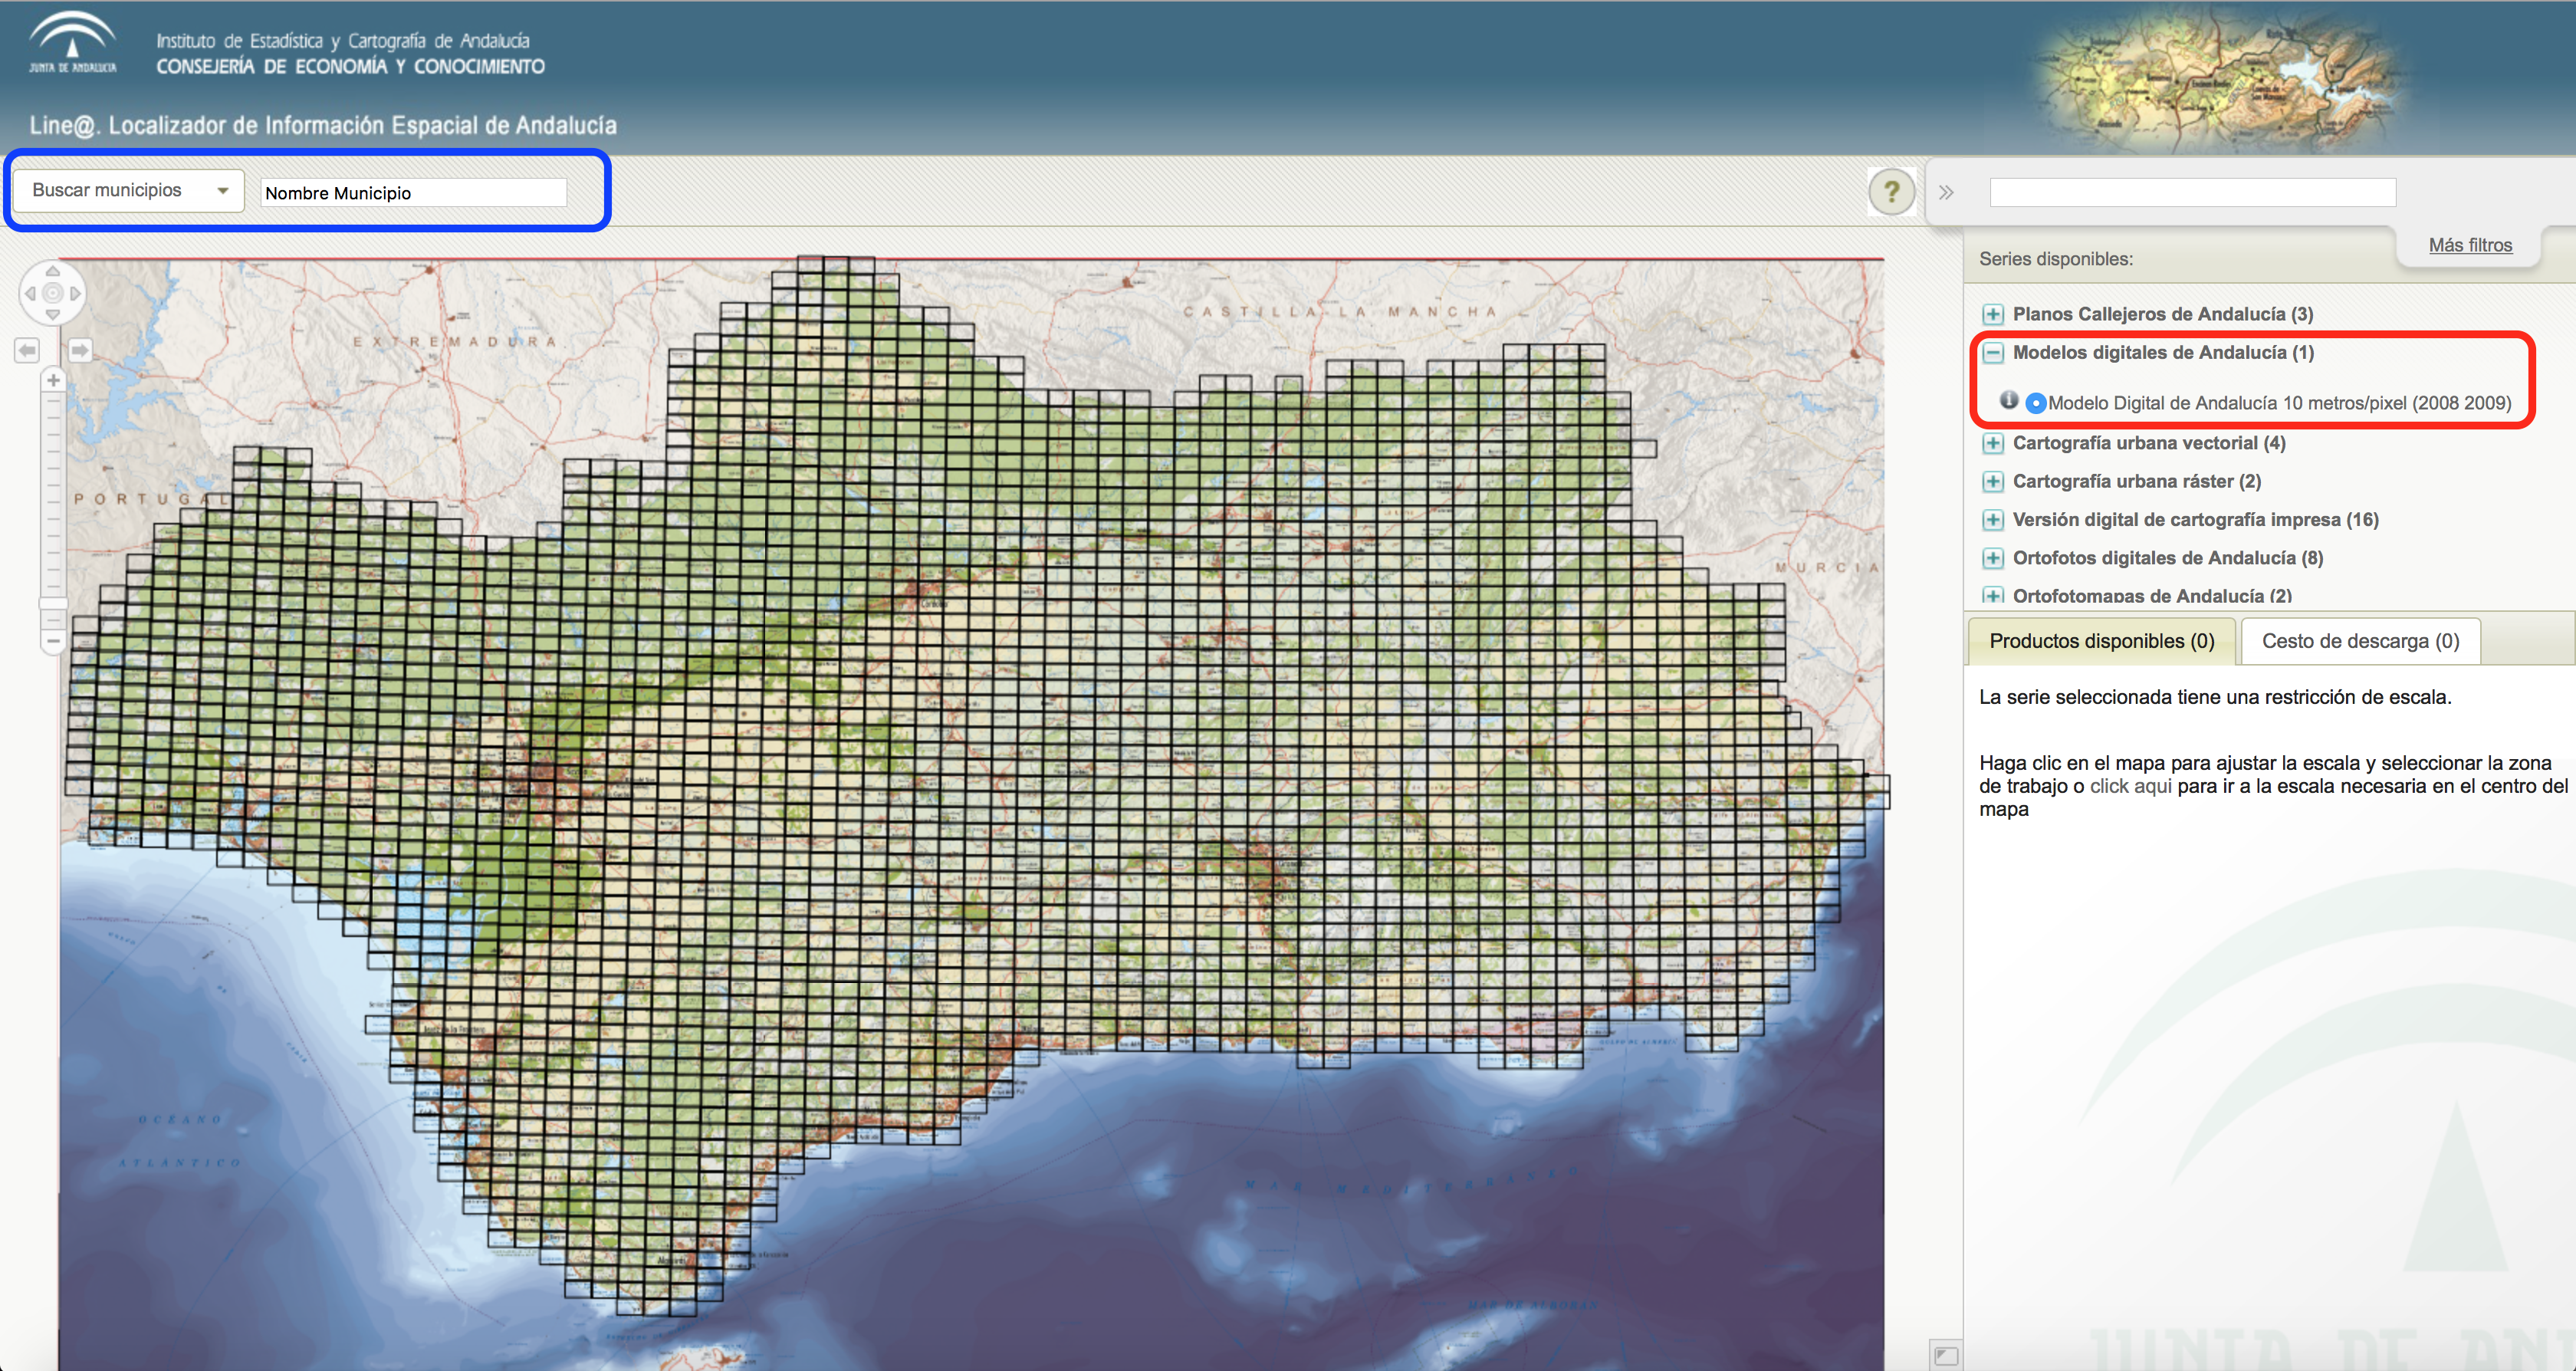
\includegraphics[height=8.5cm, angle=90,origin=c]{imagenes/capitulo2/4_Paso1-Obtencion.png}
		\caption{Portal del Instituto de Estadística y Cartografía}
		\label{fig:portal-instituto1}
	\end{figure}
	
	\begin{figure}[H]
		\centering
		\includegraphics[height=6.2cm]{imagenes/capitulo2/4_Paso2-Obtencion1.png}
		\caption{Cuadrantes perteneciente a la localidad de Chauchina}
		\label{fig:portal-instituto2}
	\end{figure}
	
	\item El fichero descargado tiene como formato \textit{Tagged Image File Format (tif)}, formato básico para el modelado de datos ráster. El contenido o visualización del fichero se muestra en la figura \ref{fig:tif}.
	
	\begin{figure}[H]
		\centering
		\includegraphics[height=6.35cm]{imagenes/capitulo2/4_Paso3-Obtencion.png}
		\caption{Archivo \textit{tif} de la zona descargada}
		\label{fig:tif}
	\end{figure}	
\end{enumerate}

Gracias a este tipo de archivo podemos generar MDT secundarios: mapas de orientación, de pendiente, cuencas visuales o sencillos archivos de sombreado (\textit{hillshade}), materia prima con la que analizar el territorio. Es por ello que, una vez descargados nuestros datos, ya podemos llevar a cabo el análisis del mapa de sombras para el MDT. Primero lo realizaremos en R, seguidamente en QGIS y, por último, veremos la interacción entre ambas, dejando documentado el proceso, para así poder hacer la evaluación y comparación entre ambas herramientas.


\section{Resumen del capítulo}





